\chapter{Results}
This chapter includes the results of the survey study (chapter \ref{ch:survey}) and the experiments with the value-sensitive rejector (chapter \ref{ch:rejector}).
%
We first present the results of the survey study as the experiments with the value-sensitive rejector depended on the outcomes of the survey study.
%

%
The goal of the survey study was to retrieve the value ratios of TP, TN, FP, FN, and rejected predictions in hate speech detection from the user's perspective.
%
We retrieved the value ratios using a scale called Magnitude Estimation (ME) and validated the ME scale by conducting a separate survey that uses a bounded scale that consists of 100 levels, called the 100-level scale.
%
The goals of the experiments with the value-sensitive rejector were finding out how the rejector behaves on different models and datasets, if ML with a reject option is beneficial for hate speech detection, and comparing the value-sensitive metric against machine metrics such as accuracy.
%

%
In section \ref{sec:results-survey-study}, we present the results of the complete  survey study that we gathered after conducting the pilot survey, and in section \ref{sec:results-rejector}, we present the results of the experiments with the value-sensitive rejector.

\section{Survey study}
\label{sec:results-survey-study}
This section presents the value ratios in section \ref{sec:results-value-ratios}, the reliability analysis in section \ref{sec:results-reliability}, the validity analysis in section \ref{sec:results-validity}, and the demographic analysis in section \ref{sec:results-demographics}.
%


\subsection{Value ratios}
\label{sec:results-value-ratios}
We collected the responses of all participants to all scenarios for both surveys (one using the ME scale and the other using the 100-level scale).
%
We plotted the results in figure \ref{fig:boxplots}.
%
\begin{figure}
    \centering
    \begin{subfigure}[b]{.9\textwidth}
        \centering
        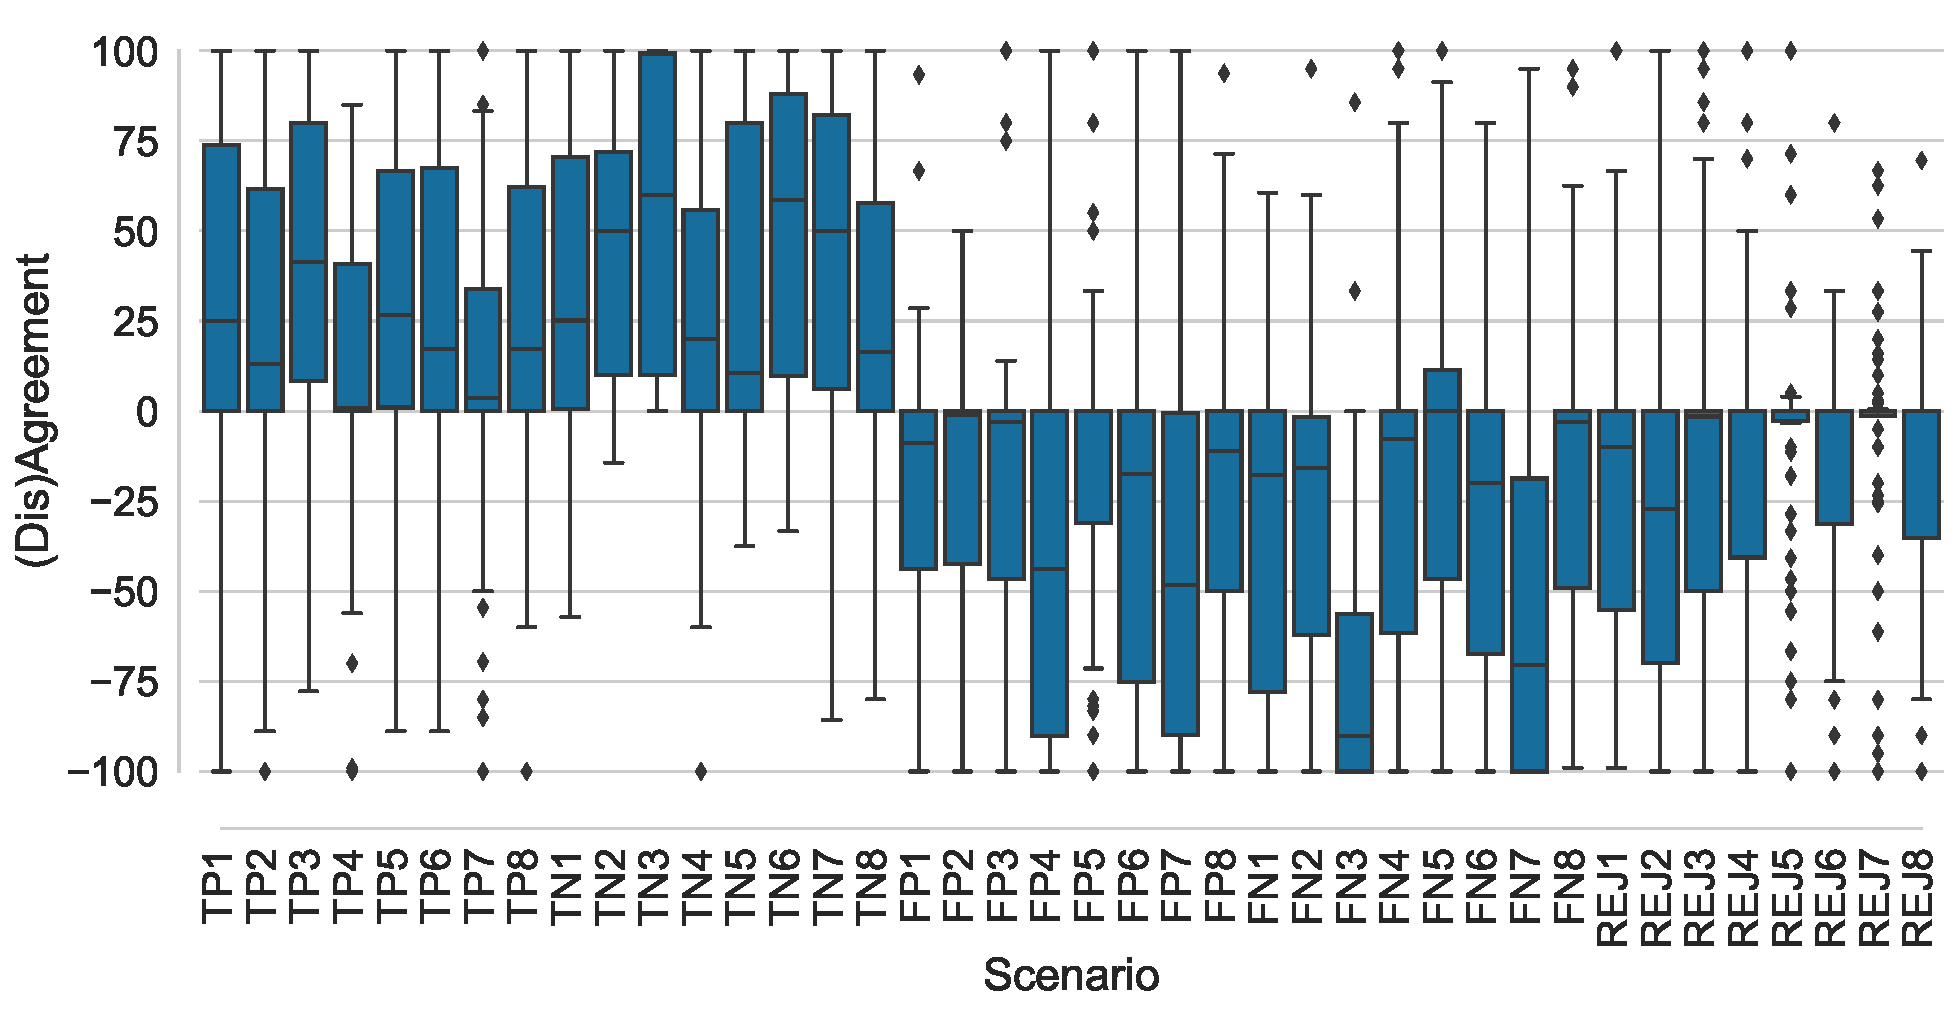
\includegraphics[width=\linewidth]{Figures/boxplots-ME.pdf}
        \caption{Scenarios rated with the ME scale.}
        \label{fig:boxplots-me}
    \end{subfigure}
    \\
    \begin{subfigure}[b]{.9\textwidth}
        \centering
        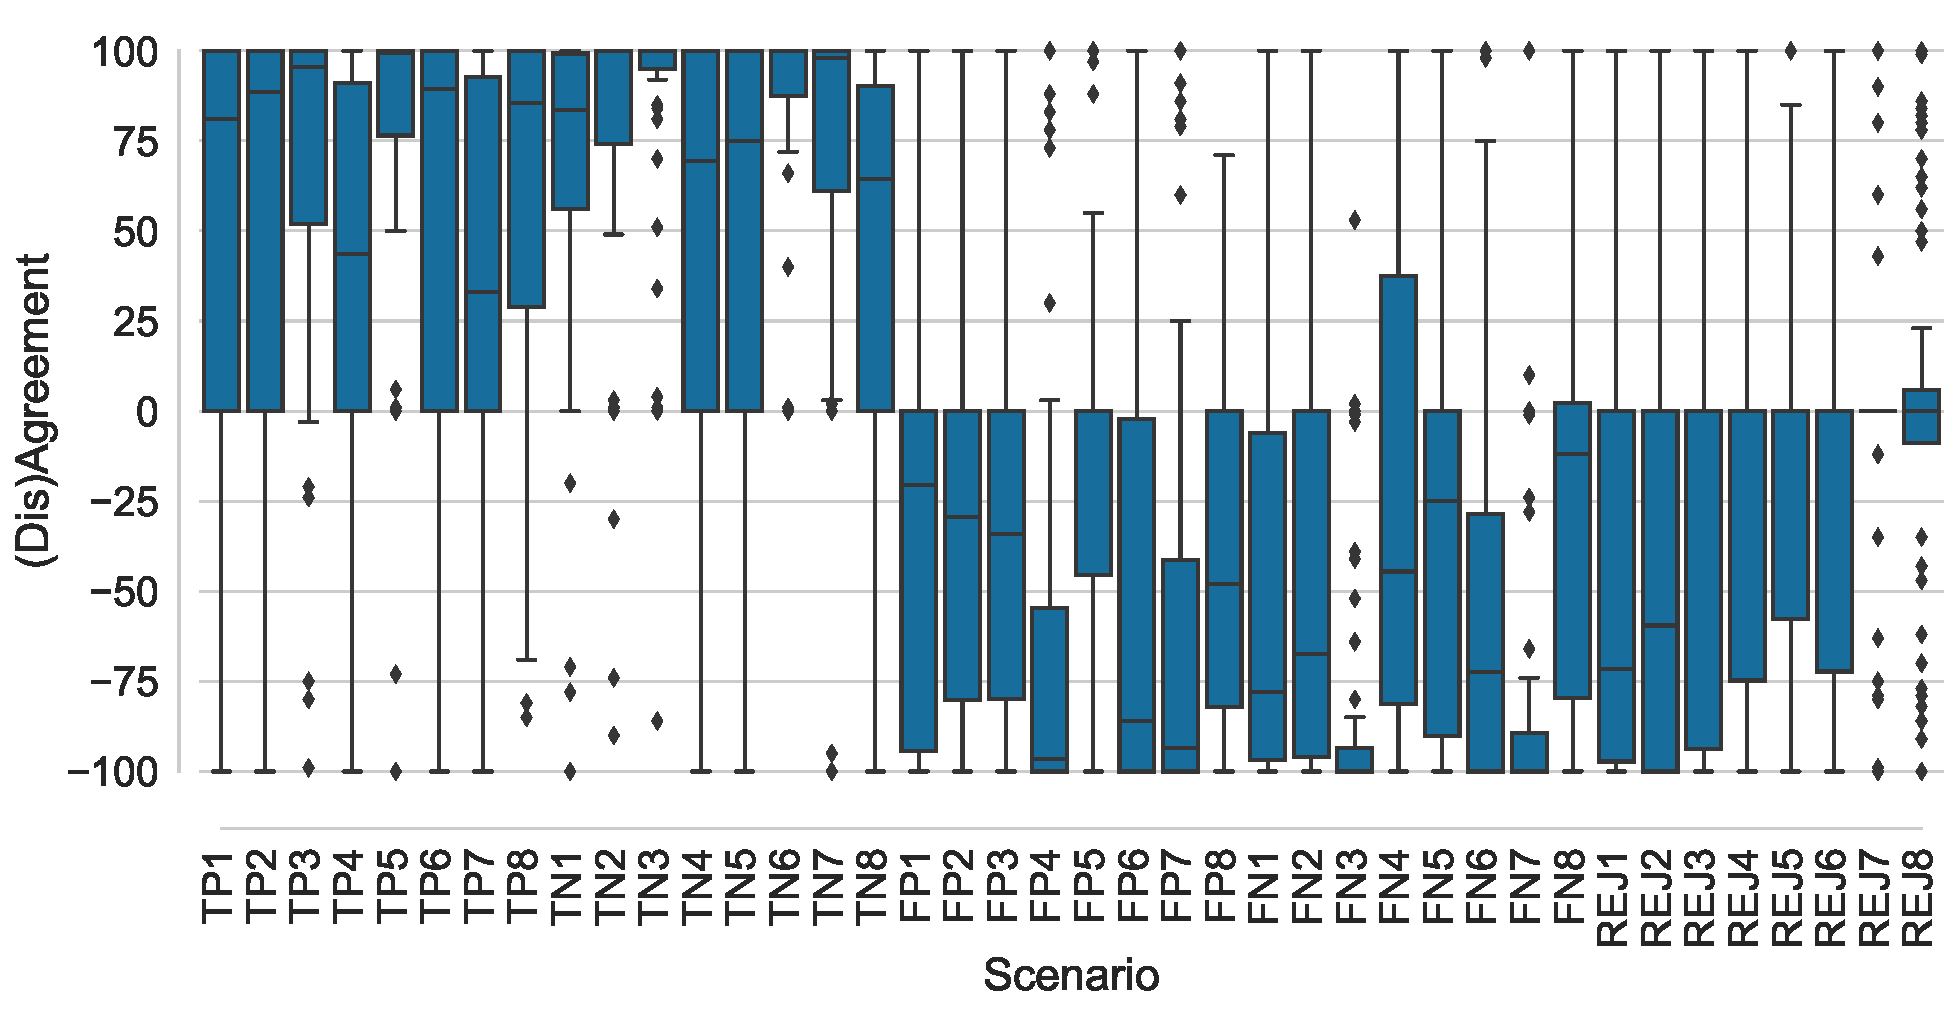
\includegraphics[width=\linewidth]{Figures/boxplots-100-level.pdf}
        \caption{Scenarios rated with the 100-level scale.}
        \label{fig:boxplots-100-level}
    \end{subfigure}
    \caption{Boxplots of the responses of all participants to all 40 scenarios.}
    \label{fig:boxplots}
\end{figure}
We calculate the value ratios by following the approach from section \ref{sec:analysis-values}.
%

%
First we calculate the median scores of all responses for each question.
%
We use the median since we found in the pilot survey that the data from both scales are highly skewed with outliers.
%
Then, we calculate the mean of all values with the same scenario type (TP, TN, FP, FN, or rejection).
%
We show the resulting value ratios in table \ref{tab:values-reliability}.
%
We

\begin{table}[t]
    \centering
    \begin{tabular}{lcccc}
        \toprule
                           & \multicolumn{2}{c}{\textbf{ME}} & \multicolumn{2}{c}{\textbf{100-level}}                                        \\
        \cmidrule(l){2-3} \cmidrule(l){4-5}
                           & $\boldsymbol{\alpha}$           & $\textbf{v}$                           & $\boldsymbol{\alpha}$ & $\textbf{v}$ \\
        \midrule
        \textbf{TP}        & 0.07                            & 18.15                                  & 0.04                  & 77.00        \\
        \textbf{TN}        & 0.10                            & 36.32                                  & 0.11                  & 86.31        \\
        \textbf{FP}        & 0.39                            & -16.69                                 & 0.07                  & -51.00       \\
        \textbf{FN}        & 0.92                            & -28.08                                 & 0.14                  & -62.43       \\
        \textbf{Rejection} & -0.31                           & -4.82                                  & 0.07                  & -16.37       \\
        \midrule
        \textbf{All}       & 0.78                            & ---                                    & 0.44                  & ---          \\
        \bottomrule
    \end{tabular}
    \caption{Krippendorff's alpha ($\alpha$) and the scenario values ($v$) for TP, TN, FP, FN, and rejection scenarios for both scales: the Magnitude Estimation (ME) and 100-level scale.}
    \label{tab:values-reliability}
\end{table}

\subsection{Reliability}
\label{sec:results-reliability}

\subsection{Validity}
\label{sec:results-validity}

\subsection{Demographics}
\label{sec:results-demographics}
\begin{table}
    \small
    \rowcolors{2}{gray!15}{white}
    \begin{tabularx}{\textwidth}{cccc|ccc}
        \toprule
        \rowcolor{white}
                      & \multicolumn{3}{c|}{\textbf{Two groups}} & \multicolumn{3}{c}{\textbf{More than two groups}}                                                                                                                                                                       \\
        \midrule
        \rowcolor{white}
                      & \multicolumn{1}{c}{\textbf{Sex}}         & \multicolumn{1}{c}{\textbf{Student}}              & \multicolumn{1}{c|}{\textbf{Continent}} & \multicolumn{1}{c}{\textbf{Nationality}} & \multicolumn{1}{c}{\textbf{Language}} & \multicolumn{1}{c}{\textbf{Ethnicity}} \\
        \midrule
        \textbf{TP1}  &                                          &                                                   &                                         &                                          &                                       &                                        \\
        \textbf{TP2}  &                                          &                                                   &                                         &                                          &                                       &                                        \\
        \textbf{TP3}  &                                          &                                                   &                                         &                                          & \cmark                                &                                        \\
        \textbf{TP4}  &                                          &                                                   &                                         &                                          &                                       &                                        \\
        \textbf{TP5}  &                                          & \cmark                                            &                                         &                                          &                                       &                                        \\
        \textbf{TP6}  &                                          &                                                   &                                         & \cmark                                   & \cmark                                &                                        \\
        \textbf{TP7}  &                                          &                                                   &                                         &                                          &                                       &                                        \\
        \textbf{TP8}  &                                          & \cmark                                            &                                         &                                          &                                       &                                        \\
        \midrule
        \textbf{TN1}  &                                          &                                                   &                                         &                                          &                                       &                                        \\
        \textbf{TN2}  &                                          &                                                   &                                         &                                          &                                       &                                        \\
        \textbf{TN3}  &                                          &                                                   &                                         &                                          &                                       &                                        \\
        \textbf{TN4}  &                                          &                                                   &                                         &                                          &                                       &                                        \\
        \textbf{TN5}  &                                          &                                                   &                                         &                                          &                                       &                                        \\
        \textbf{TN6}  &                                          &                                                   &                                         &                                          &                                       &                                        \\
        \textbf{TN7}  &                                          &                                                   & \cmark                                  &                                          &                                       &                                        \\
        \textbf{TN8}  &                                          &                                                   &                                         &                                          &                                       &                                        \\
        \midrule
        \textbf{FP1}  &                                          &                                                   &                                         &                                          &                                       &                                        \\
        \textbf{FP2}  &                                          &                                                   &                                         & \cmark                                   &                                       &                                        \\
        \textbf{FP3}  &                                          &                                                   &                                         &                                          &                                       &                                        \\
        \textbf{FP4}  &                                          &                                                   &                                         &                                          &                                       &                                        \\
        \textbf{FP5}  &                                          &                                                   &                                         &                                          &                                       &                                        \\
        \textbf{FP6}  &                                          &                                                   &                                         &                                          &                                       &                                        \\
        \textbf{FP7}  &                                          &                                                   & \cmark                                  & \cmark                                   & \cmark                                & \cmark                                 \\
        \textbf{FP8}  &                                          &                                                   &                                         &                                          &                                       &                                        \\
        \midrule
        \textbf{FN1}  &                                          &                                                   &                                         &                                          &                                       &                                        \\
        \textbf{FN2}  &                                          &                                                   &                                         &                                          &                                       &                                        \\
        \textbf{FN3}  &                                          &                                                   &                                         &                                          &                                       &                                        \\
        \textbf{FN4}  &                                          &                                                   &                                         &                                          &                                       &                                        \\
        \textbf{FN5}  &                                          &                                                   &                                         & \cmark                                   & \cmark                                &                                        \\
        \textbf{FN6}  &                                          &                                                   &                                         & \cmark                                   &                                       &                                        \\
        \textbf{FN7}  &                                          &                                                   &                                         &                                          & \cmark                                &                                        \\
        \textbf{FN8}  &                                          & \cmark                                            &                                         &                                          &                                       &                                        \\
        \midrule
        \textbf{REJ1} &                                          &                                                   &                                         & \cmark                                   & \cmark                                &                                        \\
        \textbf{REJ2} &                                          &                                                   &                                         &                                          &                                       &                                        \\
        \textbf{REJ3} &                                          &                                                   &                                         &                                          &                                       &                                        \\
        \textbf{REJ4} &                                          &                                                   & \cmark                                  & \cmark                                   & \cmark                                & \cmark                                 \\
        \textbf{REJ5} &                                          &                                                   &                                         &                                          & \cmark                                &                                        \\
        \textbf{REJ6} &                                          &                                                   &                                         &                                          &                                       &                                        \\
        \textbf{REJ7} &                                          &                                                   &                                         &                                          &                                       & \cmark                                 \\
        \textbf{REJ8} &                                          &                                                   &                                         &                                          &                                       &                                        \\
        \bottomrule
    \end{tabularx}
    \caption{\textbf{Individual}: overview of the statistically significant differences between different groups of participants for each individual scenario in the ME survey. A check or cross indicates that we found significant or no significant differences between the groups, respectively. We use the non-parametric Mann-Whitney U test for the \emph{sex}, \emph{student}, and \emph{continent} features and the non-parametric Kruskal-Wallis test for the \emph{nationality}, \emph{language}, and \emph{ethnicity} features.}
    \label{tab:results-differences-ind}
\end{table}

\begin{table}
    \small
    \centering
    \begin{tabular}{cccc|ccc}
        \toprule
                     & \multicolumn{3}{c}{\textbf{Two groups}} & \multicolumn{3}{c}{\textbf{More than two groups}}                                                                                                                                                                       \\
        \midrule
                     & \multicolumn{1}{c}{\textbf{Sex}}        & \multicolumn{1}{c}{\textbf{Student}}              & \multicolumn{1}{c}{\textbf{Continent}} & \multicolumn{1}{c}{\textbf{Nationality}} & \multicolumn{1}{c}{\textbf{Language}}  & \multicolumn{1}{c}{\textbf{Ethnicity}} \\
        \midrule
        \textbf{TP}  & 0.302                                   & \cellcolor[HTML]{EFEFEF}\textbf{0.032}            & 0.286                                  & 0.218                                    & 0.109                                  & 0.242                                  \\
        \textbf{TN}  & 0.726                                   & 0.379                                             & 0.204                                  & 0.190                                    & 0.216                                  & 0.281                                  \\
        \textbf{FP}  & 0.699                                   & 0.933                                             & 0.073                                  & \cellcolor[HTML]{EFEFEF}\textbf{0.020}   & \cellcolor[HTML]{EFEFEF}\textbf{0.040} & \cellcolor[HTML]{EFEFEF}\textbf{0.037} \\
        \textbf{FN}  & 0.961                                   & 0.150                                             & 0.847                                  & 0.478                                    & 0.438                                  & 0.584                                  \\
        \textbf{REJ} & 0.835                                   & 0.625                                             & 0.496                                  & 0.271                                    & 0.103                                  & 0.068                                  \\
        \bottomrule
    \end{tabular}
    \caption{\textbf{Aggregated}: an overview of the statistical differences between different groups of participants for various demographic characteristics for each aggregated scenario type in the ME survey. Each cell contains the p value of either the Mann-Whitney U test for two groups or the Kruskal-Wallis test for more than two groups. The grey cells with bold text indicate significant statistical differences between the groups for that feature and scenario type.}
    \label{tab:results-differences-grp}
\end{table}

\section{Value-sensitive rejection}
\label{sec:results-rejector}
\todo[inline]{Explain that the metric conditions still hold if we set $V_{tp}$ and $V_{tn}$ to 0}
